% ======================================================================

\chapter{Raceline Optimization}
\label{chap:opt}

Lo studio di questa tesi si è concentrato a trovare una soluzione al seguente problema: \textit{data una
mappa, trovare la sua raceline globale ottima, secondo un criterio scelto}. Il
criterio di ottimizzazione principale, in questi casi, è il tempo di percorrenza del tracciato, ovvero il
\textit{lap time}.

Le porzioni interessanti di un circuito da gara sono le \textit{curve}: ne esistono di diversi tipi e
altrettanti modi per affrontarle in base al tipo; trovare una percorso ottimo, in questo senso, è un
compito complesso e il percorso più breve non coincide necessariamente con quello che richiede meno
tempo, a causa delle curve che riducono la velocità media. Una possibile strategia per mantenere alta la
velocità in curva è quella di percorrere la traiettoria con la curvatura minore. Questo approccio,
tuttavia, non prende in considerazione una sequenza di curve e la velocità di uscita da una curva. Il
percorso ottimo in termini di tempo, quindi, è un compromesso tra queste due strategie, ovvero quella che
minimizza la distanza percorsa mantenendo alta la velocità nelle curve ed eventualmente anche in uscita
da esse.

Trovare la raceline ottima è generalmente un'operazione preliminare alla gara, dunque \textit{non può
considerare} eventuali avversari o ostacoli dinamici; per questo motivo viene calcolata nell'assunzione
di un \textit{singolo robot} sul tracciato.
Tuttavia non è utile solo nel contesto considerato: la raceline globale, avendo una visione intera sulla
mappa, può essere sfruttata da un local o behavioural planner come linea guida.

% ================== Le Curve ==========================================
\section{Le curve}
Le principali complessità di un circuito di cui l'ottimizzazione si occupa è come affrontare le curve.\\
Caratteristica principale di una curva è il suo \textit{raggio}: un raggio maggiore corrisponde a
velocità più alte e viceversa; inoltre, si distinguono il raggio esterno e quello interno e la loro
differenza risulta nell'ampiezza del circuito in quel punto.
Esistono anche caratteristiche di natura tridimensionale, come la variazione dell'altezza e
l'inclinazione, tuttavia non sono state oggetto di studio in questa tesi dal fatto che il contesto di
F1TENTH non include questa variabilità, come invece accade nelle gare di F1.

In linea generale, una curva può essere suddivisa in \textit{quattro sequenze} principali, come mostrato
in figura \ref{fig:geom-raceline}:
\begin{enumerate}
	\item approccio e decelerazione;
	\item inizio della curva;
	\item raggiunta dell'apice;
	\item uscita della curva e accelerazione.
\end{enumerate}
Anche la traiettoria, dato che segue una curva, può essere definita con un raggio che può essere
\textit{costante} o \textit{variabile} dall'inizio della curva fino alla fine.

\begin{figure}[H]
	\begin{center}
		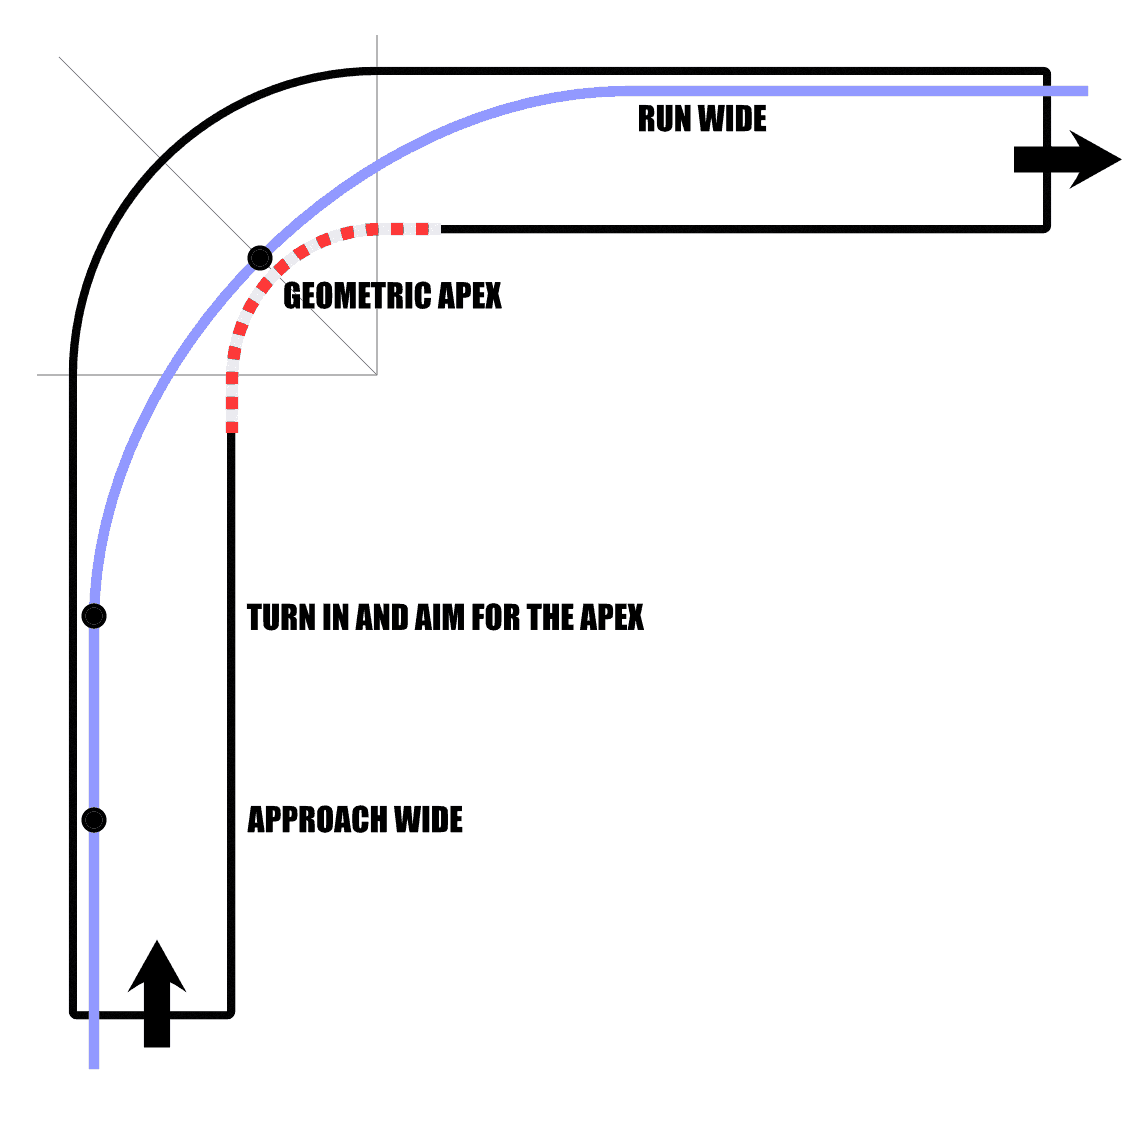
\includegraphics[width=0.65\textwidth]{geometric-apex.png}
	\end{center}
	\caption{Rappresentazione delle fase di una raceline geometrica per una curva a destra \cite{drivingfast}}
	\label{fig:geom-raceline}
\end{figure}

\paragraph{Raceline geometrica}
L'approccio più semplice e immediato per affrontare una curva genera una raceline che prende il
nome di \textit{raceline geometrica}. La strategia prevede queste sequenze, rappresentate in figura
\ref{fig:geom-raceline}:
\begin{enumerate}
	\item approccio largo e verso l'esterno del circuito;
	\item sterzata verso il centro del raggio interno della curva;
	\item uscita larga e verso l'esterno del circuito.
\end{enumerate}
Si tratta, quindi, di una raceline a raggio \textit{costante}.\\
I principali vantaggi di questo approccio rispetto alla raceline ottima sono la sua semplicità, sia in
termini di modellazione sia in termini di computazione, e la possibilità di mantenere un'alta velocità
durante la curva. Tuttavia, la raceline geometrica ha importanti svantaggi quali una decelerazione
prematura all'entrata della curva, una accelerazione ritardata all'uscita e la possibilità di ritrovarsi
in uno stato svantaggiato per affrontare la prossima curva, nel caso di curve in sequenza.

Dunque, la raceline ottimale non dovrebbe tener conto solamente della singola curva ma eventualmente
anche di quelle successive: per estensione, quindi, deve essere considerato tutto il circuito.

\paragraph{Raceline ottimale}
Al contrario della raceline geometrica, non è possibile definire a priori le sequenze da seguire come
fatto in precedenza, proprio perché dipende dalle caratteristiche della curva.
Riprendendo come esempio la curva in figura \ref{fig:geom-raceline}, la raceline ottimale -- ovvero quella
che riesce ad eseguire la curva nel minor tempo possibile -- tarda il più possibile l'inizio della curva
per mantenere più velocità all'entrata, decelera più velocemente e ha una virata più stretta e con un
apice più distante da quello geometrico, così facendo si ha la possibilità di aver più tempo per
accelerare di nuovo all'uscita della curva con la possibilità di mantenere una traiettoria più centrata
rispetto al circuito.

In figura \ref{fig:cmp-lines} vi è una comparazione grafica tra le due raceline.\\
La raceline ottima, inoltre, adegua la traiettoria di uscita in base alla curva successiva, se presente,
in modo tale da affrontarla anch'essa nel modo ottimale. Si nota la distinzione in figura
\ref{fig:cmp-opt-lines}.

\begin{figure}[H]
	\begin{minipage}[c]{0.45\textwidth}
		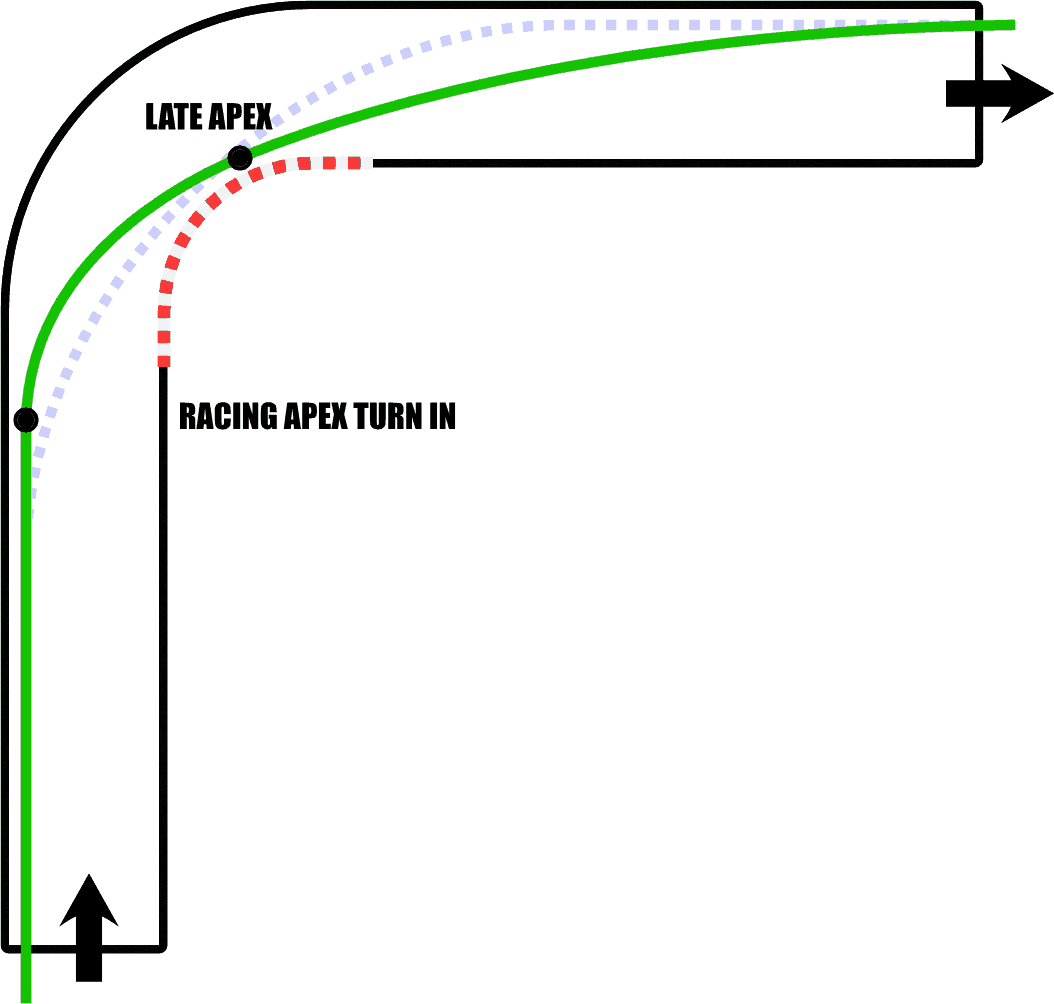
\includegraphics[width=0.80\textwidth]{comparing-lines.png}
		\caption{Comparazione tra raceline ottimale, in verde, e raceline geometrica, in blu
		tratteggiato \cite{drivingfast}}
		\label{fig:cmp-lines}
	\end{minipage}\hfill
	\begin{minipage}[c]{0.45\textwidth}
		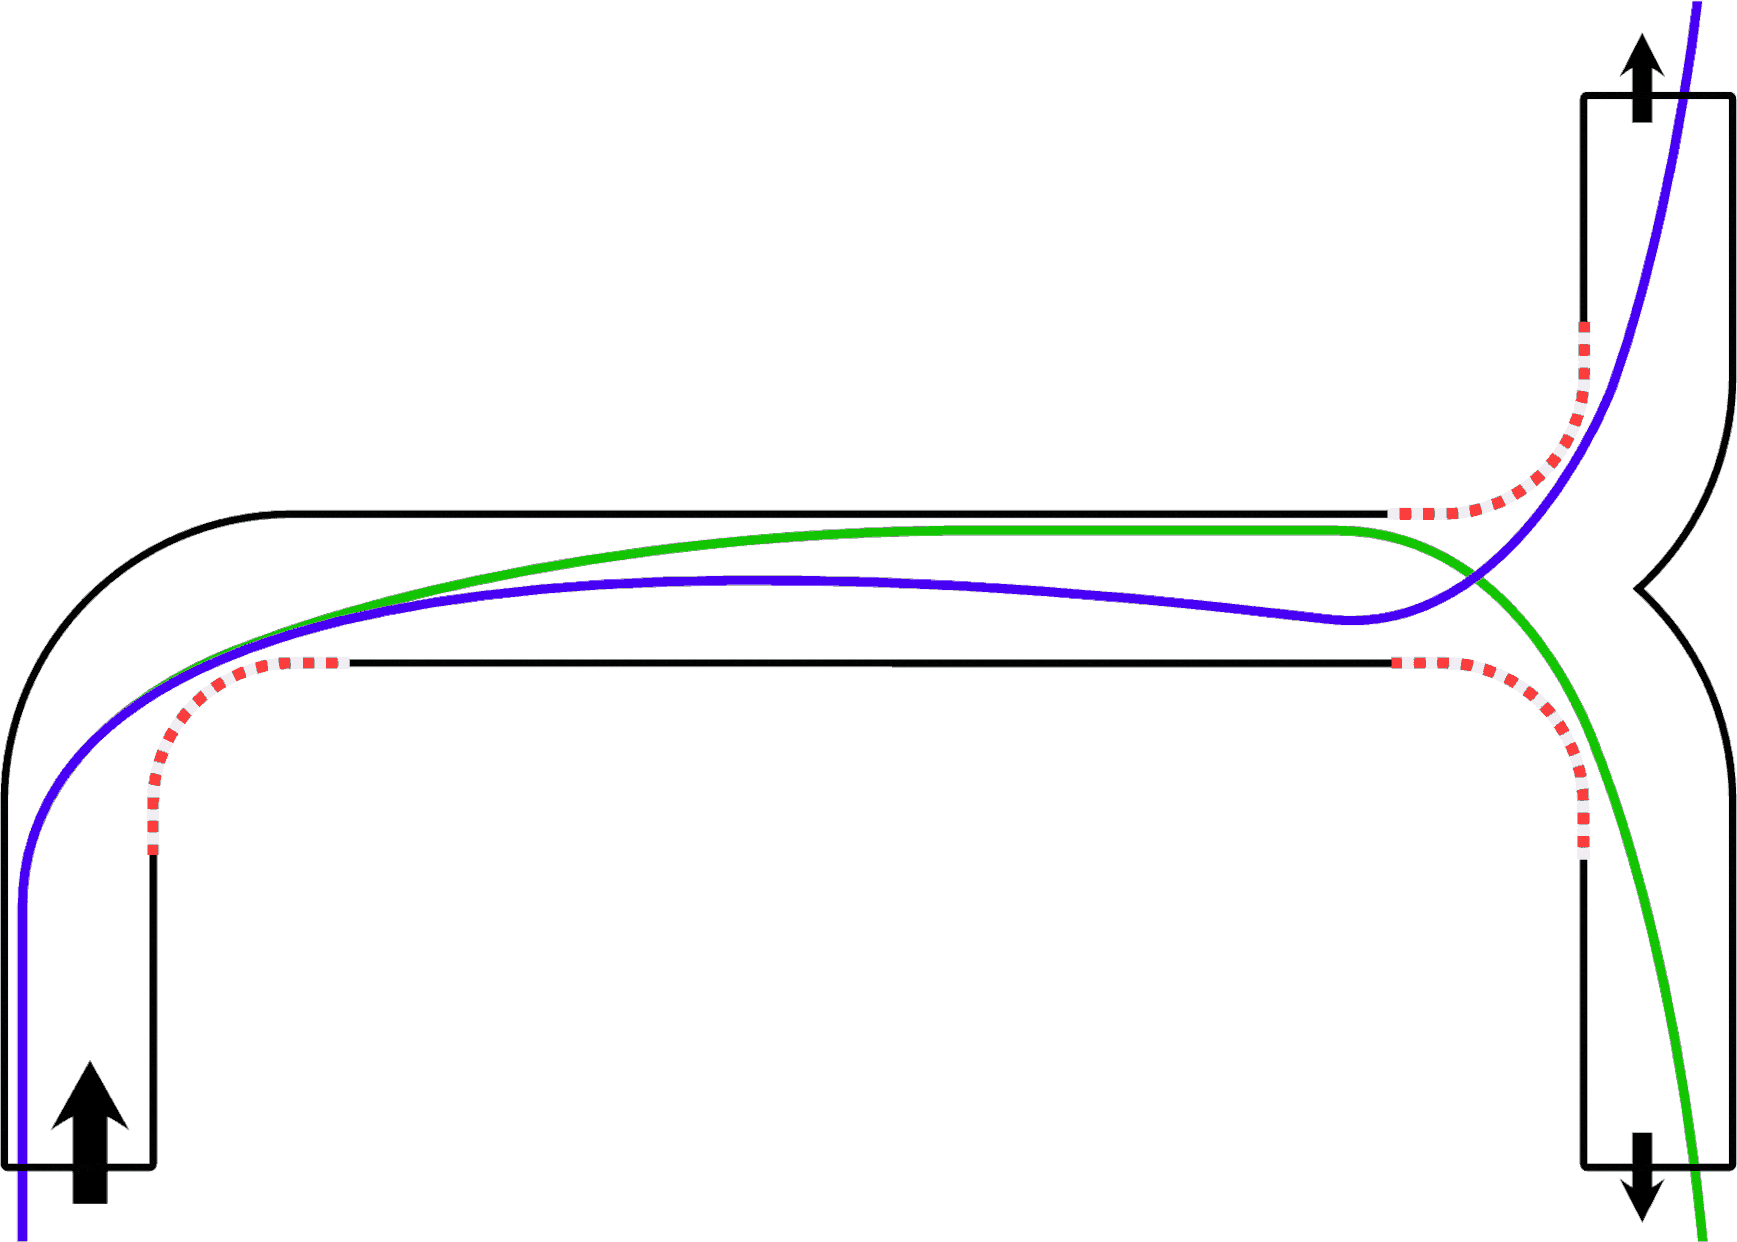
\includegraphics[width=1\textwidth]{multiple-corners.png}
		\caption{\raggedright Confronto tra raceline ottime con due curve distinte in
		sequenza \cite{drivingfast}}
		\label{fig:cmp-opt-lines}
	\end{minipage}
\end{figure}


% ================== Descrizione del problema ==========================
\section{Descrizione del problema}
% Il lavoro è stato basato su questa repo \url{https://github.com/CL2-UWaterloo/Raceline-Optimization}.
% fonti: L22 Raceline-Optimization slide

Di seguito si presentano alcune definizioni più formali dei termini utilizzati precedentemente e il
processo di generazione del percorso ottimo secondo un certo criterio.

\bigskip
\noindent In questa tesi sono state implementate e analizzate tre strategie differenti:
\begin{itemize}
	\setlength\itemsep{0em}
	\item Percorso più breve  -- \textit{shortest path};
	\item Curvatura minima -- \textit{minimum curvature};
	\item Tempo minimo -- \textit{minimum time}.
\end{itemize}

\noindent Il problema in questione è un problema di ricerca su due variabili: il percorso effettivo sulla mappa e
la velocità da mantenere per ogni punto del percorso. Queste due variabili assieme definiscono la
\textit{traiettoria} o \textit{raceline}, in inglese.\\
I vincoli applicati alla ricerca sono due: i limiti dinamici del veicolo, per esempio quanta forza G il
veicolo riesce a sostenere in sterzata, e gli ostacoli statici, rappresentati dai bordi del circuito.

\bigskip
\noindent Il problema viene suddiviso in due sotto-problemi, ovvero risolvere singolarmente la ricerca sulle due
variabili in gioco. Si distinguono quindi, in sequenza:
\begin{enumerate}
	\setlength\itemsep{0em}
	\item Generazione del percorso secondo i vincoli desiderati -- \hyperref[sec:path-models]{\textit{path
		planning}}
	\item Calcolo della velocità sul percorso generato -- \hyperref[sec:velocity-plan]{\textit{velocity
		planning}}
\end{enumerate}
In particolare, il path planning, almeno per quanto riguarda le prime due strategie, viene modellato come
un problema di programmazione quadratica geometrica (Geometric QP), che ha i vantaggi di richiedere pochi
parametri e di essere computazionalmente veloce; esistono anche altri tipi di algoritmi di ottimizzazione
basati su evoluzione, come CMA-ES. Il velocity planning può essere risolto con algoritmi a stato
quasi-stazionario come l'algoritmo forward-backward. Un ulteriore metodo per il velocity planning per il
tempo più breve è descritto in \textit{"Minimum-time speed optimization over a fixed path"}
\cite{lipp2014minimum}.

Per quanto riguarda la terza strategia, i due sotto-problemi devono essere risolti contemporaneamente
usando algoritmi di controllo ottimale, questi hanno la possibilità di includere ulteriori vincoli, come
per esempio limitazioni al consumo di energia o considerare l'attrito delle ruote per diversi terreni e
condizioni meteo.\cite{christ2021time} Sono algoritmi con modelli dinamici dell'auto più completi e
fedeli alla realtà che raccolgono nel problema diverse variabili, per questo sono più complessi e
richiedono più sforzo computazionale, ma hanno il vantaggio di essere più realistici nel risultati
rispetto alle loro controparti modellate in problemi di programmazione quadratica.

\paragraph{Definizione di spline \cite{olausson2021optimal} \cite{globalplanning-lec}}
\label{par:spline-def}
Un percorso, per poter essere computato da una macchina, deve necessariamente essere discretizzato in
punti, detti \textit{samples}.
Tuttavia è necessaria una descrizione matematica del tracciato: questa viene formulata con l'uso delle
\textit{spline}. Una spline è una funzione definita a pezzi da un'insieme di polinomi dello stesso grado
il cui scopo, in questo contesto, è quello di interpolare dei punti, ovvero i samples, in modo tale che
la funzione sia continua fino ad un dato ordine.

Una spline, per poter rappresentare un percorso che deve essere seguito da un'auto, è necessario che
rispetti alcuni vincoli, ovvero:
\begin{enumerate}
	\item L'inizio di un polinomio deve essere un punto di discretizzazione, un sample;
	\item La fine di un polinomio deve essere il sample successivo all'inizio;
	\item L'orientamento alla fine di una funzione deve essere uguale all'orientamento della funzione
	      successiva;
	\item La curvatura alla fine di una funzione deve essere uguale alla curvatura della funzione
	      successiva;
\end{enumerate}
I primi due vincoli sono garantiti dal fatto che la spline interpola i sample, per gli ultime due è
necessario calcolare la derivata prima e seconda del polinomio in quei punti. I polinomi di grado tre
offrono, quindi, una buona rappresentazione del percorso perché garantiscono la calcolabilità delle
derivate prime e seconde per ogni punto del dominio.

Il dominio di ogni polinomio viene normalizzato per la distanza tra il punto di partenza e quello di fine
dal parametro $t$, dove $t = 0$ indica il punto di inizio e $t = 1$ il punto di fine.
Sia $f_i(t) = a_i + b_i t + c_i t^3 + d_i t^3$ il polinomio che ha come inizio il sample all'indice $i$,
l'immagine \ref{fig:spline} mostra graficamente una spline e i vincoli associati.

\begin{figure}
	\begin{center}
		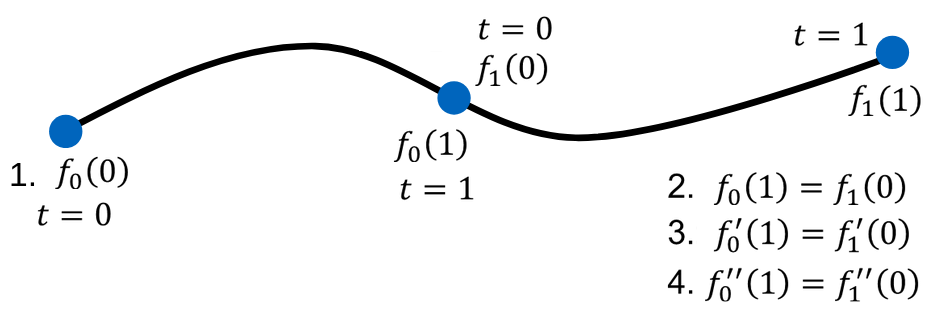
\includegraphics[width=0.95\textwidth]{spline.png}
	\end{center}
	\caption{Esempio di spline formata da due polinomi e vincoli associati \cite{lection22}}
	\label{fig:spline}
\end{figure}
Il calcolo dei valori delle $x$ e delle $y$ avviene separatamente ma usando gli stessi metodi, di
seguito, quindi, verranno descritti solo la formulazione per $x$.
Matematicamente i vincoli sopra descritti vengono formulati come:
\begin{enumerate}
	\item $t = 0 \quad a_i = x_i$
	\item $t = 1 \quad a_i + b_i + c_i + d_i = x_{i+1}$
	\item $t = 1\ \text{e}\ t = 0 \quad b_i + 2 c_i + 3 d_i - b_{i+1} = 0$
	\item $t = 1\ \text{e}\ t = 0 \quad 2 c_i + 6 d_i - 2 c_{i+1} = 0$
\end{enumerate}
dove per il 3. e 4. punto vengono rispettivamente ricavati dalla differenza \\
$f'_i(1) - f'_{i+1}(0)$ e $f''_i(1) - f''_{i+1}(0)$

% Un esempio dell'uso di una spline per interpolare dei punti è mostrato in figura \ref{fig:spline}

\paragraph{Definizione di centerline}
\label{par:centerline}
La centerline, o reference line, è il percorso che è equidistante dai bordi del circuito. Viene
discretizzato in punti di egual distanza tra loro e si registrano le distanze ai bordi destro e sinistro,
così da formare una line immaginaria, ortogonale alla reference line, che unisce i due punti. L'immagine
\ref{fig:centerline-ex} ne mostra un esempio grafico.

La linea centrale di riferimento è necessaria agli algoritmi di ottimizzazione come punto di partenza per
trovare la soluzione ottima.
La distanza dei samples è un parametro dell'algoritmo e deve essere decisa in base al caso d'uso, come
approfondito al paragrafo \ref{par:tuning}.

\begin{figure}[h]
	\begin{center}
		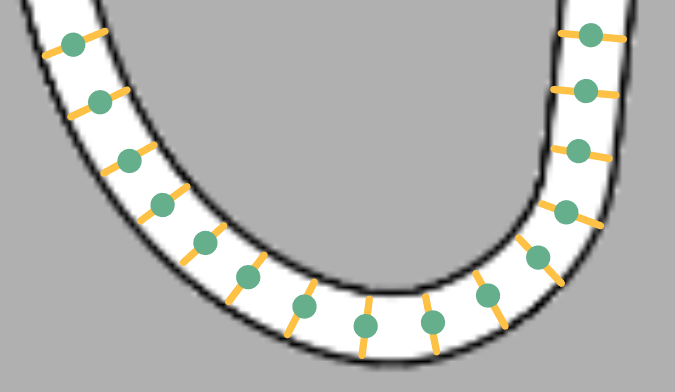
\includegraphics[width=0.65\textwidth]{centerline-ex.png}
	\end{center}
	\caption{La figura mostra la rappresentazione discreta della centerline (i punti verdi) e le linee
		immaginarie (quelle gialle) che uniscono, ortogonalmente rispetto alla centerline, i bordi
		del circuito}
		\label{fig:centerline-ex}
\end{figure}

\paragraph{Definizione di raceline}
\label{par:raceline}
I samples della raceline vengono calcolati a partire da quelli delle centerline "muovendoli" sulla linea
immaginaria che unisce i due bordi. Formalmente:
\[
	\overrightarrow{r_i} = \overrightarrow{p_i} + \alpha_i \overrightarrow{n_i}
\]
dove il sample $i$ della raceline $r$, descritto dal vettore $\overrightarrow{r_i}$, viene traslato di un
fattore $a_i$ lungo il vettore $\overrightarrow{n_i}$, ovvero la linea che unisce i bordi del circuito.
La figura \ref{fig:raceline-def} rappresenta graficamente questo processo.

\begin{figure}[h]
	\begin{center}
		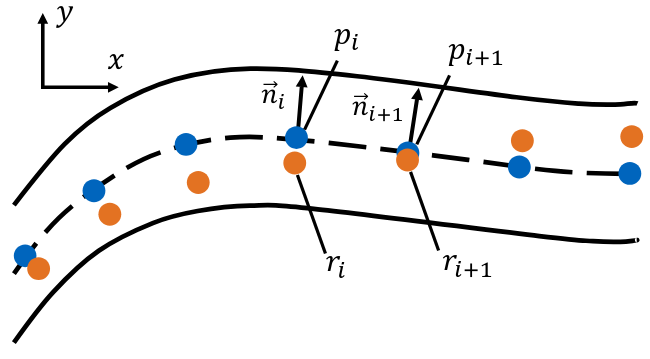
\includegraphics[width=0.75\textwidth]{raceline-def.png}
	\end{center}
	\caption{Rappresentazione grafica della raceline, dove i punti blu rappresentano i samples della
		centerline, mentre quelli arancioni sono quelli della raceline, traslati di un certo fattore lungo i
		vettori $n$ corrispondenti. \cite{lection22}}
	\label{fig:raceline-def}
\end{figure}

È necessario, inoltre, imporre un vincolo sul fattore $a$ in modo tale che non venga prodotto un sample
al di fuori del circuito o che non permetta al robot di passare perché troppo vicino ai bordi.
Formalmente:
\begin{equation}
	a_i \in [ -w_{tr\_left, i} + \frac{w_{veh}}{2}, w_{tr\_right, i} - \frac{w_{veh}}{2}]
	\label{eq:a_constr}
\end{equation}
dunque, dato un indice $i$, il fattore $a$ deve rientrare nel range definito tra la distanza del circuito
a sinistra $w_{tr\_left}$ del sample della centerline dello stesso indice e la distanza a destra
$w_{tr\_right}$ aggiustato per la larghezza del veicolo $w_{veh}$.

% ================== Path Planning =====================================
\section{Path planning}
\label{sec:path-models}
Ora verranno esaminate più in dettaglio il modello dei problemi di QP
geometrico per le strategie di percorso più breve e minor curvatura.

La programmazione quadratica è un processo che risolve problemi di ottimizzazione matematica descritti da
funzioni quadratiche. L'obiettivo è quello di trovare un vettore che minimizzi o massimizzi il valore di
una funzione obiettivo preservando contemporaneamente dei vincoli, descritti da disequazioni.

\paragraph{Percorso più breve}\cite{race-model}\cite{globalplanning-lec}
Il modello in questione deve descrivere il percorso più breve, ovvero che abbia la distanza minore tra i
samples. Un sample della raceline viene formulato come:
\[
	\overrightarrow{P_i} =
	\begin{bmatrix}
		x_{r,i} + a_i(x_{l,i} - x_{r,i}) \\
		y_{r,i} + a_i(y_{l,i} - y_{r,i})
	\end{bmatrix} =
	\begin{bmatrix}
		x_{r,i} + a_i\Delta_{x,i} \\
		y_{r,i} + a_i\Delta_{y,i}
	\end{bmatrix}
\]
ovvero, il punto più a destra del segmento $i$-esimo ortogonale alla centerline spostato sullo stesso per
un fattore $a$. Nella figura \ref{fig:short-path-expl} ne viene mostrato un esempio.\\
La distanza tra un sample e il suo successivo può essere descritta, quindi, come:
\[
	\Delta P_{x, i} = \overrightarrow{P}_{i+1} - \overrightarrow{P_i} = \begin{bmatrix}
		x_{r,i+1} - x_{r,i} + a_{i+1}\Delta_{x,i+1} - a_i\Delta_{x, i} \\
		y_{r,i+1} - y_{r,i} + a_{i+1}\Delta_{y,i+1} - a_i\Delta_{y, i}
	\end{bmatrix}
\]
Le variabili da trovare è il vettore di $a$ da applicare ai samples, dunque:
\[
	\begin{aligned}
		min\ [a_i \dots a_N] & \sum_{i=1}^{N} (\Delta P_{x,i})^2                          \\
		\text{subj. to}\     & a_i \in [a_{i, min}, a_{i, max}] \quad \forall 1 <= i <= N
	\end{aligned}
\]
dove il vincolo per $a_i$ è lo stesso descritto nella formula \ref{eq:a_constr}.

\begin{figure}[h]
	\begin{center}
		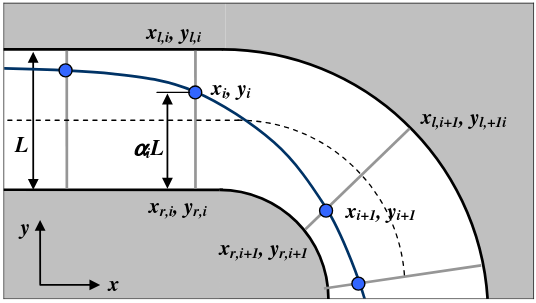
\includegraphics[width=0.65\textwidth]{short-path-expl.png}
	\end{center}
	\caption{Rappresentazione grafica della descrizione matematica di un sample. \cite{race-model}}
	\label{fig:short-path-expl}
\end{figure}

\paragraph{Minima Curvatura}
La formulazione del modello è identica a differenza, ovviamente, della funzione obiettivo che deve
descrivere la curvatura della raceline, il modello, quindi, viene definito come:
\[
	\begin{aligned}
		min\ [a_i \dots a_N] & \sum_{i=1}^{N} \kappa_i^2                                  \\
		\text{subj. to}\     & a_i \in [a_{i, min}, a_{i, max}] \quad \forall 1 <= i <= N
	\end{aligned}
\]
dove $\kappa_i$ è la curvatura della funzione in un sample $i$, definita come:
\[
	\kappa_i = \frac{{x'_i} {y''_i} - y'_i x''_i}{({x'_i}^2 + {y'_i}^2)^\frac{3}{2}}
\]
che elevata al quadrato:
\[
	\kappa_i^2 = \frac{{x'_i}^2 {y''_i}^2 - 2 x'_i x''_i y'_i y''_i + {y'_i}^2 {x''_i}^2}{({x'_i}^2 + {y'_i}^2)^3}
\]

% ================== Velocity Planning =================================
\section{Velocity planning}
\label{sec:velocity-plan}
Come citato precedentemente, il calcolo della velocità per ogni sample può essere calcolato con
l'algoritmo \textit{forward-backward}, che ha il vantaggio di essere semplice, veloce e sufficientemente
accurato.

L'algoritmo assume che il robot venga guidato ai suoi limiti fisici per ogni punto del percorso, quindi
si ha che l'accelerazione longitudinale dipende dai limiti del motore e dall'azione frenante dei freni,
mentre l'accelerazione laterale è limitata dalle forze massime trasmissibili degli pneumatici.

Ad alto livello, l'algoritmo si può riassumere in:
\begin{enumerate}
	\item Si genera una prima stima della velocità basandosi sulla massima accelerazione laterale per la
	      curvatura di ogni sample;
	\item Si riducono le stime alla velocità massima consentita per quei sample che la superano;
	\item \textbf{Forward}: si itera sui samples e, se non si sono superati i limiti fisici del robot, si
		applica una possibile accelerazione longitudinale, altrimenti
	\item \textbf{Backward}: si itera sui samples e si applica una possibile decelerazione longitudinale.
\end{enumerate}
In particolare per gli ultimi due punti la velocità al punto successivo viene calcolata come segue:
\begin{enumerate}

	\item \raggedright Si calcola l'accelerazione laterale data la curvatura per quel sample:\\
	      \centering $a_{y,i} = v_i^2 \cdot \kappa_i$ 

	\raggedright
	\item Si determina il potenziale rimanente per l'accelerazione longitudinale:\\
	      \begin{center}
			  $a_{x,i} = a_{x,max} \sqrt{\displaystyle 1- \left(\frac{a_{y,i}}{a_{y,max}}\right)^2}$
		  \end{center}

	\item Si può calcolare quindi la velocità al punto successivo assumendo un'accelerazione costante per
		la distanza $l_i$ tra un sample e quello successivo:\\
		\centering $v_{i+1} = \sqrt{v_i^2 + 2 \cdot a_{x,i} \cdot l_i}$
\end{enumerate}
